\documentclass{article}

\usepackage{amsmath}
\usepackage{amssymb}
\usepackage{amsthm}
\usepackage{parskip}
\usepackage{fullpage}
\usepackage{hyperref}
\usepackage{pgfplots}
\usepackage{wrapfig}
\usepackage{bettelini}
\usetikzlibrary{calc}

\hypersetup{
    colorlinks=true,
    linkcolor=black,
    urlcolor=blue,
    pdftitle={DifferentialEquations},
    pdfpagemode=FullScreen,
}

\renewcommand\qedsymbol{\(\blacksquare\)}

\newtheorem*{theorem1}{Theorem}
\newtheorem*{theorem2}{Theorem}
\newtheorem*{theorem3}{Theorem}
\newtheorem*{theorem4}{Theorem}
\newtheorem*{theorem5}{Theorem}
\newtheorem*{theorem6}{Theorem}

\title{Differential Equations}
\author{Paolo Bettelini}
\date{}

\begin{document}

\maketitle
\tableofcontents
\pagebreak

\section{Definition}

Differential equations are equations where the solution is a function
or a set of functions.

\subsection{Order}

The \textit{order} of a differential equation is the largest derivative present in the
differential equation

\subsection{Types}

\textit{Ordinary differential equations} are equations with only
ordinary derivatives in them, whilst \textit{partial differential equations}
have partial derivatives in them.

\subsection{Linearity}

A differential equation is said to be linear if it can be written as
\[
    \sum_n a_n(t) \frac{d^n}{dt^n}y(t)=g(t)
\]
where there are no products of the function \(y(t)\) and its derivatives,
\(y(t)\) or its derivative do not occur to any power other than the first power
and \(y(t)\) or any of its derivative are composed with another function.

\section{First-Order Differential Equations}

A first-order differential equation is a differential equation in the form
\[
    y'(t)=f(t,y(t))
\]
where \(f\) is given.

The equation is said to be \textit{linear}
if \(f\) is linear on the second argument.
\[
    y'(t)=a(t)y(t) + b(t)
\]
The equation is also said to be \textit{constant}
if \(a\) and \(b\) are also constant.

\pagebreak

\subsection{Constant Coefficients Differential Equations}

\begin{theorem1}
    The general solution to the constant differential equation
    \[
        y' = ay+b,
        \quad a \neq 0
    \]
    is given by
    \[
        y(t)=Ce^{at}-\frac{b}{a}, \quad C \in \mathbb{R}
    \]
\end{theorem1}
\begin{proof}
    Let's first consider the case when \(b=0\),
    \[
        y'=ay
    \]
    We divide both sides by \(y\) and simplify
    \[
        \frac{y'}{y}=a
        \implies
        \ln|y|'=a
        \implies
        \ln|y|=at+c_0
    \]
    concluding that
    \[
        y = \pm e^{at+c_0}=\pm e^{c_0} \cdot e^{at} = Ce^{at}
    \]
    Now let's consider \(b \in \mathbb{R}\)
    \[
        y'=a\left(y+\frac{b}{a}\right)
        \implies
        \left(y + \frac{b}{a}\right)' = a\left(y + \frac{b}{a}\right)
    \]
    Note that \(\frac{d}{dx}\left(\frac{b}{a}\right)=0\) \\
    Denoting \(\tilde{y}=y+\frac{b}{a}\), we have
    \[
        \tilde{y}=a\tilde{y}
    \]
    which has solution \(Ce^{at}\), hence
    \begin{align*}
        y+\frac{b}{a}&=Ce^{at} \\
        y &= Ce^{at} - \frac{b}{a}
    \end{align*}
\end{proof}

\pagebreak

It is important to note that we solved the equation by turning
it into a total derivative, which is simple to integrate \((\ln|y|'=a)\).
This function is called a \textit{potential function} \((\psi)\) and it's how
the equation is transformed into a total derivative
\[
    y'=ay+b \rightarrow \psi(t, y(t))'=0
\]
In this case
\[
    \psi = \ln|y| - at
\]

\paragraph{The Integrating Factor Method}
The integrating factor method is a method for solving linear
differential equations.
\\
We will prove the theorem again using this method.
\begin{proof}
    We choose an integrating factor to be a function \(\mu\) such that
    \[
        \mu'=-a\mu
    \]
    By solving this differential equation we get
    \[
        \frac{\mu'}{\mu} = -a
        \implies
        \ln|\mu| = -at+C
        \implies
        \mu(t) = Ce^{-at}
    \]
    Now we multiply the equation by \(\mu\)
    \begin{align*}
        y'-ay&=b \\
        y'\mu - \mu ay &= b\mu \\
        y'\mu + \mu' y &= b \mu \\
        (\mu y)' &= \mu b
    \end{align*}
    Now choosing \(C=1\)
    \begin{align*}
        \left(e^{-at}y\right)'&=be^{-at} \\
        \left(e^{-at}y\right)'&=\left(-\frac{b}{a}e^{-at}\right)' \\
        \left(e^{-at}y+\frac{b}{a}e^{-at}\right)' &= 0 \\
        \left[\left(\frac{b}{a} + y\right)e^{-at}\right]' &= 0
    \end{align*}
    Now the differential equation is a total derivative of the potential function,
    which in this case in
    \[
        \psi(t, y) = \left(\frac{b}{a} + y\right)e^{-at}
    \]
    This is easy to integrate
    \[
        \left(\frac{b}{a} + y\right)e^{-at} = C
        \implies
        y = Ce^{at} - \frac{b}{a}
    \]
\end{proof}

\pagebreak

\subsection{Constant Coefficients Differential Equations with Initial Point}

We want to constraint the equation such that it has an unique solution
rather than infinite solutions.
\[
    y' = ay + b, \quad y(t_0) = y_0
\]

\begin{theorem2}
    The general solution to the ordinary constant differential equation
    \[
        y' = ay + b,
    \]
    with a given point
    \[
        y(t_0) = y_0
    \]
    is given by
    \[
        y(t)=\left(y_0 + \frac{b}{a}\right) e^{a(t-t_0)}- \frac{b}{a},
        \quad a \neq 0
    \]
\end{theorem2}
\begin{proof}
    Starting from the general solution of a constant ordinary differential equation
    \[
        y(t_0) = y_0 = Ce^{at_0} - \frac{b}{a}
    \]
    meaning that
    \[
        C = \left(y_0 + \frac{b}{a}\right) e^{-at_0}
    \]
    this constraints out result to
    \begin{align*}
        y(t) &= Ce^{at} - \frac{b}{a} \\
             &= \left(y_0 + \frac{b}{a}\right) e^{-at_0} e^{at} - \frac{b}{a} \\
             &= \left(y_0 + \frac{b}{a}\right) e^{a(t-t_0)} - \frac{b}{a}
    \end{align*}
\end{proof}

\subsection{Linear Coefficients Differential Equations}

An ordinary linear differential equation with variable coefficients is defined as
\[
    y' = a(t)y(t) + b(t)
\]
Where \(a\) and \(b\) are continuous functions.
The solution to the linear equation with constant coefficients still applies
if \(\frac{b}{a}\) is constant.

\begin{theorem3}
    The general solution to the differential equation
    \[
        y' = a(t)y(t) + b(t)
    \]
    is given by
    \[
        y(t)=Ce^{A(t)} + e^{A(t)} \int e^{-A(t)} b(t)\, dt
    \]
    where \(A(t)=\int a\,dt\), \(c\in\mathbb{R}\) and \(a\) and \(b\) are
    continuous.
\end{theorem3}
\begin{proof}
    Let's start by letting \(b(t)=0\)
    \[
        y' = ay
        \implies
        \frac{y'}{y}=a
        \implies
        \ln|y|'=a
        \implies
        \ln|y|=\int a\,dt
    \]
    concluding that
    \[
        y = \pm e^{A+c_0}=\pm e^{c_0} \cdot e^{A} = Ce^A
    \]
    where \(A=\int a\, dt\).
    \\
    As previosuly, we choose an integrating factor \(\mu\) such that
    \[
        -a\mu = \mu'
    \]
    By solving this differential equation we get
    \[
        \frac{\mu'}{\mu} = -a
        \implies
        \ln|\mu| = -A+C
        \implies
        \mu(t) = Ce^{-A}
    \]
    And by choosing \(C=1\) we have
    \[
        \mu(t) = e^{-A(t)}
    \]
    Now we multiply our equation by the integrating factor
    \begin{align*}
        y' - ay &= b \\
        y'\mu - a\mu y &= \mu b \\
        y' \mu + \mu' y &= \mu b \\
        \left(y \mu\right)' &= \mu b \\
        \left(e^{-A(t)}y\right)' &= e^{-A(t)}b \\
        e^{-A(t)}y &= \int e^{-A(t)}b \,dt + C \\
        y(t) &= Ce^{A(t)} + e^{A(t)} \int e^{-A(t)}b \,dt
    \end{align*}
\end{proof}

\subsection{Linear Coefficients Differential Equations with Initial Point}

A linear differential equation with variable coefficients and an initial point is given by
\[
    y'(t) = a(t)y(t) + b(t), \quad
    y(t_0) = y_0
\]

\begin{theorem4}
    The general solution to the differential equation
    \[
        y'=a(t)y(t)+b(t)
    \]
    where \(a\) and \(b\) are continuous functions, with a given point
    \[
        y(t_0)=y_0
    \]
    is given by
    \[
        y(t)=y_0 e^{A(t)}+e^{A(t)} \integral[t_0][t][e^{-A(s)}b(s)][s]
    \]
\end{theorem4}
\begin{proof}
    % pag 18
\end{proof}

\pagebreak

\subsection{Bernoulli Equation}

The Bernoulli equation has the form
\[
    y' = p(t)y + q(t)y^n
\]

\begin{theorem5}
    The general solution of the Bernoulli equation is the general
    solution of the linear equation
    \[
        v' = -(n-1)p(t)v-(n-1)q(t)
    \]
    where
    \[
        v = \frac{1}{y^{n-1}}
    \]
\end{theorem5}
\begin{proof}
    They idea is to transform this equation into a simplier
    linear first-order equation. \\
    Start by dividing both sides by \(y^n\)
    \[
        \frac{y'}{y^n} = \frac{p(t)}{y^{n-1}} + q(t)
    \]
    Let
    \[
        v = y^{-(n-1)}, 
        \quad
        v' = -(n-1)y^{-n}y'
    \]
    Thus
    \[
        -\frac{v'}{n-1} = \frac{y'(t)}{y^n(t)}
    \]
    By substituting we get
    \begin{align*}
        -\frac{v'}{n-1} &= p(t)v + q(t) \\
        v' &= -(n-1)p(t)v-(n-1)g(t)
    \end{align*}
\end{proof}

\pagebreak

\subsection{Separable equations}

Separable equations are equations that can be solved by integrating both sides.
This doesn't generally work with first-order linear equations.
A separable equation has the form
\[
    h(y)y'=g(t)
\]
\begin{theorem6}
    A separable differential equation has an implicit solution
    \[
        H(y(t)) = G(t) + C
    \]
    where
    \begin{align*}
        H(y) = \int h(s)\,ds
        ,\quad
        G(t) = \int g(t)\,dt
    \end{align*}
\end{theorem6}
\begin{proof}
    Start by integrating both sides of the equation
    \[
        \int h(y(t))y'(t)\,dt =
        \int g(t)\,dt + C
    \]
    Now substitute for
    \[
        s=y(t),
        \quad
        ds=y'(t)\,dt
    \]
    meaning
    \[
        \int h(s)\, ds = 
        \int g(t)\,dt
    \]
    which could be written as
    \[
        H(y) = G(t) + C
    \]
\end{proof}

\pagebreak

\subsection{Exact equations}

Consider a differential equation with the form
\[
    M(x,y)+N(x,y)\frac{dy}{dx}=0
\]
Then, the equation is \textit{exact} if there exist a continuously
differentiable function \(\Psi(x,y)\) such that
\[
    \frac{\partial \Psi}{\partial x} = M(x,y)
    \quad \text{and} \quad
    \frac{\partial \Psi}{\partial y} = N(x,y)
\]
We can then rewrite the differential equation as
\[
    \frac{\partial \Psi}{\partial x}+\frac{\partial \Psi}{\partial y} \frac{dy}{dx}=0
\]
Using the multi variable chain rule it can be reduced to
\[
    \frac{d}{dx}\left( \Psi(x,y(x)) \right) = 0
\]
We can clearly see that here the derivative is equal to \(0\), meaning that
the function must be a constant. This gives us an implicit solution
\[
    \Psi(x,y)=C
\]

\pagebreak

\subsection{Homogeneous equations}

A \textit{homogenous} equation has the form
\[
    \frac{dy}{dx} = F(\frac{y}{x})
\]
We use the substitution
\[
    v=\frac{y}{x}
\]
Note that
\begin{align*}
    y' &= (xv)' = v+yv' \\
    &= F(v)
\end{align*}
We then have
\begin{align*}
    v+xv'&=F(v) \\
    xv'&=F(v)-v \\
    \frac{v'}{F(v)-v}&=\frac{1}{x}
\end{align*}

This is a separable equation. Thus, an implicit solution is given by
\[
    \integral[\frac{1}{F(v)-v}][v]=\ln|x|+C
\]

\pagebreak

\subsection{Slope Field}

A slope field or directional field is a field to visualize
solutions to a first-order differential equation.

\begin{wrapfigure}{l}{7.5cm}
    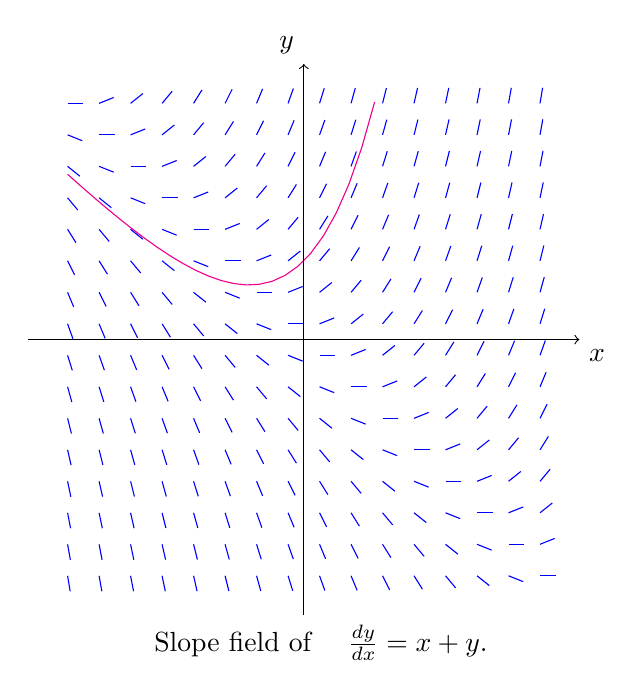
\begin{tikzpicture}[declare function={f(\x,\y)=\x+\y;}]
        \def\xmax{3} \def\xmin{-3}
        \def\ymax{3} \def\ymin{-3}
        \def\nx{15}
        \def\ny{15}
        
        \pgfmathsetmacro{\hx}{(\xmax-\xmin)/\nx}
        \pgfmathsetmacro{\hy}{(\ymax-\ymin)/\ny}
        \foreach \i in {0,...,\nx}
            \foreach \j in {0,...,\ny}{
                \pgfmathsetmacro{\yprime}{f({\xmin+\i*\hx},{\ymin+\j*\hy})}
                \draw[blue,shift={({\xmin+\i*\hx},{\ymin+\j*\hy})}] 
                (0,0)--($(0,0)!2mm!(.1,.1*\yprime)$);
            }
        
        % a solution y=(yo+1)e^x-x-1
        \def\yo{1}
        \draw[magenta] plot[domain=\xmin:.9] (\x,{(\yo+1)*exp(\x)-\x-1});
        
        \draw[->] (\xmin-.5,0)--(\xmax+.5,0) node[below right] {\(x\)};
        \draw[->] (0,\ymin-.5)--(0,\ymax+.5) node[above left] {\(y\)};
        
        \draw (current bounding box.south) node[below]
        {Slope field of \quad \(\frac{dy}{dx}=x+y\).};
    \end{tikzpicture}
\end{wrapfigure}

\phantom{ } \\

This field is obtained by picking points on the plane. \\
For each point \((x,y)\) we know that the slope \((\frac{dy}{dx})\)
is \(x + y\). \\
This means that if a solution passes through \((x,y)\), then its slope is \(x+y\). \\
The red curve shows a solution.

\wrapfill

\subsection{Euler's Method}

Euler's method is a technique for solving a 
first-order differential equation numerically given a point of the solution.
\\
Starting at the known solution point \(A_0\), we take small steps the direction
of the slope field. As the length of the steps \(s \to 0\)
we approach the solution to the equation. \\
%The angle of the slope is given by
%\[
%    \theta = \tan^{-1}\left(\frac{dy}{dx}\right)
%\]
%so each step gives the sequence of points
%\[
%    A_n = A_{n-1} \cdot s \left(\cos(\theta), \sin(\theta)\right)
%\]

\pagebreak

\section{Second-Order Differential Equations}

A second-order differential equation has the form
\[
    y''(t)+a(t)y'(t)+b(t)y(t)=f(t)
\]
if \(f(t)=0\) then the equation is said to be \textit{homogeneous}.

% skipped https://tutorial.math.lamar.edu/Classes/DE/IntroSecondOrder.aspx

\pagebreak

\section{Laplace Transform}

Given a piecewise continuous function \(f(t)\), the Laplace transform
is defined as
\[
    \mathcal{L}\{f(t)\}= \integral[0][\infty][e^{-st}f(t)][t]=F(s)
\]

\subsection{Properties of the Laplace Transform}

It is easy to see that given \(f(t)\) and \(g(t)\)
\[
    \mathcal{L}\{af(t)+bg(t)\} = a\mathcal{L}\{f(t)\} + b\mathcal{L}\{g(t)\}
\]
for any constants \(a\) and \(b\).

\subsection{Inverse Laplace Transform}

The Inverse Laplace Transform is defined as
\[
    {\mathcal{L}}^{-1} \{F(s)\}= f(t)
\]

\subsection{Properties of the Inverse Laplace Transform}

Given the Laplace transforms \(F(s)\) and \(G(s)\)
\[
    {\mathcal{L}}^{-1} \{aF(s)+bG(s)\} =
    a{\mathcal{L}}^{-1}\{F(s)\} +
    b{\mathcal{L}}^{-1}\{G(s)\}
\]
for any constants \(a\) and \(b\).

\subsection{Heaviside function}

A consider a function in the form \(H(t-c)f(t-c)\) where \(H\) is the
Heaviside step function, meaning \(f(t)\) is shifted by \(c\) and is \(0\) for \(t < c\).

\begin{align*}
    \mathcal{L}\{H(t-c)f(t-c)\} &=
    \integral[0][\infty][e^{-st}H(t-c)f(t-c)][t] \\
    &= \integral[c][\infty][e^{-st}f(t-c)][t]
\end{align*}
Now substitue for \(u=t-c\)
\begin{align*}
    \integral[0][\infty][e^{-s(u+c)}f(u)][u]
    &= \integral[0][\infty][e^{-su}e^{-cs}f(u)][u] \\
    &= e^{-cs} \integral[0][\infty][e^{-su}f(u)][u]
\end{align*}

\pagebreak

Concluding that

\[
    \mathcal{L}\{H(t-c)f(t-c)\} =
    e^{-cs}F(s)
    \quad
    \text{and}
    \quad
    {\mathcal{L}}^{-1}\{e^{-cs}F(s)\} =
    H(t-c)f(t-c)
\]

\subsection{Laplace Transform of derivatives}

Let \(f'\), \(f''\), \(\cdots\), \(f^{(n-1)}\) be continuous functions
and \(f^{(n)}\) a piecewise continuous functions. Then,
\[
    \mathcal{L}\{f^{(n)}\} =
    s^n \mathcal{L}\{f\} -
    \sum_{k=1}^n s^{n-k}f^{(k-1)}(0)
\]

\subsection{Solving Initial value problems}

Given an initial value problem differential equation, we can apply the Laplace
transform on both sides of the equation. After applying the initial conditions
(\(y(0), y'(0), \cdots\)), the differential equation is transformed into an algebraic equation.

Note that if the initial conditions are not expressed as  \(y(0), y'(0), \cdots\),
we need to first make a change of variable.

We can then isolate \(\mathcal{L}\{y\}\) in the equation and get
\[
    \mathcal{L}\{y\} = M
\]
Then apply the inverse Laplace transform to solve the equation
\[
    y={\mathcal{L}}^{-1}\{M\}
\]

% from https://tutorial.math.lamar.edu/Classes/DE/IVPWithNonConstantCoefficient.aspx

\end{document}

% reference https://users.math.msu.edu/users/gnagy/teaching/ode.pdf